\chapter{Testes e Resultados} \label{chap:testes}

\section*{}

Neste capítulo é apresentada a fase de testes, especificando as suas características e algumas conclusões obtidas.

\section{Planeamento de Testes}

Para efetuar os testes da aplicação decidiu-se que estes seriam feitos em ambiente real, com utilizadores reais. Estes testes foram realizados no decorrer do quotidiano dos utilizadores, sendo feitos em paralelo com a utilização normal dos transportes públicos por eles realizada. Pretendeu-se com estes testes avaliar a relevância e perceção do conceito de bilhética móvel aplicado aos transportes públicos, bem como analisar a usabilidade e consistência da aplicação de bilhética móvel desenvolvida.
\\Os testes decorreram durante o período de 14 dias (duas semanas completas), entre os dias 5 e 18 de junho de 2013. O processo de seleção foi levado a cabo pela STCP, tentando obter o máximo de heterogeneidade em termos de vários fatores demográficos (género, idade, ocupação). Foram selecionados inicialmente 37 utilizadores para a realização dos testes.\cite{stcp}
\\As condições de participação eram as seguintes:

\begin{itemize}
\item Possuir telemóvel com sistema operativo Android com versão 2.2 (Froyo) ou superior;
\item Cumprir o período de testes delineado, do início ao fim;
\item Carregar normalmente os cartões Andante e validá-los assim que se dê início a uma viagem. Em simultâneo, comprar os mesmos bilhetes através do telemóvel e validá-los antes do início de cada viagem. Isto significa que os utilizadores deverão utilizar os dois sistemas (cartão Andante e telemóvel) ao mesmo tempo;
\item Os encargos com a compra de bilhetes através do sistema Andante ficam a cargo do utilizador. Relativamente à compra de bilhetes com o telemóvel não haverá qualquer encargo adicional pois ser-lhes-á fornecida uma conta fictícia com  \euro 70 para utilizarem em títulos de viagem;
\item Cada utilizador deverá efetuar pelo menos 5 validações por semana. As validações do telemóvel deverão coincidir com as validações do cartão Andante que estiverem a utilizar, em termos de data, hora e local;
\item Caso os utilizadores sejam fiscalizados pelos Fiscais da STCP deverão mostrar o bilhete Andante e o telemóvel. Se o bilhete Andante não estiver válido para a viagem em questão, os Fiscais efetuarão as diligências normais;
\item Os utilizadores deverão estar disponíveis para responderem a um inquérito inicial e a uma entrevista no final dos testes.
\end{itemize}

\section{Inquérito Inicial}

Com a realização do inquérito inicial pretendeu-se perceber o perfil dos utilizadores, a nível de utilização de dispositivos móveis, utilização de transportes públicos e confiança em pagamentos móveis. Dos 37 utilizadores selecionados, 26 responderam ao inquérito inicial, sendo 10 do sexo feminino e 16 do sexo masculino, com idades compreendidas entre os 21 e 68 anos e idade média a rondar os 34 anos.
\\A maioria dos utilizadores possuem um \emph{smartphone} há 6 meses ou mais, sendo que apenas 3 o possuem há menos de 6 meses. A partir desta informação podemos concluir que são pessoas que têm alguma familiaridade com o uso e funcionamento dos \emph{smartphones}, facilitando a adaptação à aplicação.
\\Em relação ao tipo de aplicações que utilizam com mais frequência, as redes sociais surgem, sem surpresa, em primeiro plano (21), sendo seguidas por transportes (13), jogos (13), música (16), navegação (19), fotos e vídeo (16) e meteorologia (17) em níveis semelhantes. Sendo que a maioria destas aplicações requer acesso à Internet, não se mostrou problemática a necessidade de aceder à Internet por parte da aplicação, visto que a maioria dos utilizadores possui plano de dados nos tarifários que utilizam.
\\São todos utilizadores frequentes dos transportes públicos e na maior parte das vezes (92\%) realizam viagens urbanas, sendo o autocarro o meio de transporte mais utilizado por todos. Cerca de metade dos utilizadores efetuam transbordo intermodal (autocarro-metro; autocarro-comboio; etc.).
\\A maior parte dos utilizadores compra os seus títulos nas máquinas de venda automática (18) ou através dos agentes Payshop e CTT (11) e rede multibanco (9) e utilizam tanto cartão multibanco (15) como dinheiro (11) para efetuar o pagamento. A maioria (23) compra assinatura mensal, devido a que com uma utilização frequente se apresenta como uma solução mais barata e também por possuírem descontos sociais.
\\Os serviços adicionais que mais utilizam são a consulta de horários (25) e a consulta de mapas da rede de transportes (15), sendo o acesso a esta informação feito maioritariamente através da página \web dos operadores (23) mas também nas paragens e estações (18).

~\\Em geral, são poucas as perdas ou extravios dos cartões Andante e é ainda complicado, em algumas situações, compreender o número de zonas necessárias para efetuar determinada viagem. Apesar de considerarem fácil a compra de títulos nas máquinas de venda automática, é frequente não terem dinheiro trocado para efetuar a compra dos títulos, sendo obrigados a realizar o pagamento com cartão multibanco. A necessidade de terem de se deslocar a uma loja física para renovar a assinatura mensal é vista com algum desagrado porque muitas vezes têm de fazer essa deslocação propositadamente, para além do inconveniente das filas existentes no início/final de cada mês.
\\O sistema atual de validação não apresenta qualquer dificuldade e a capacidade de poder, a qualquer instante, saber o tempo restante do título de viagem atual seria uma mais-valia para o sistema Andante. Uma outra funcionalidade que consideram bastante útil é saber qual a paragem até à qual podem viajar com o título atual. Para além disso, a possibilidade de poderem carregar consigo títulos de diferentes tipologias (Z2, Z3, etc.) é vista com bons olhos, pois o sistema atual (ClickZ) não funciona na perfeição. Atualmente, é possível carregar diferentes tipologias no cartão mas é validado sempre o mais recente, isto é, um cartão com títulos Z2, após a compra de títulos Z3, apenas se pode voltar a usar os títulos Z2 quando todos os títulos Z3 tiverem sido gastos. Outras funcionalidades consideradas úteis seriam o acesso ao histórico de viagens e de compras de títulos.
\\Um dado importante, já referenciado noutros estudos, é o facto de ser bastante mais provável deixarem o cartão Andante em casa do que o telemóvel.

~\\Em relação à compra de títulos de viagem através do telemóvel, bem como à sua utilização quando o serviço estiver disponível, os utilizadores mostram-se bastante recetivos, considerando este método de pagamento útil e seguro, para além de não interferir com a utilização habitual do telemóvel, nem com os seus estilos de vida. No entanto, têm algumas reticências no que toca aos problemas que possam surgir no caso de ficarem sem rede ou sem bateria, bem como falhas da aplicação e demonstram alguma preocupação com o facto de poderem cometer erros na compra dos títulos.

~\\À semelhança da compra, em relação à validação de títulos de viagem através do telemóvel, bem como à sua utilização quando o serviço estiver disponível, os utilizadores mostram-se bastante recetivos, considerando este método de validação útil e seguro, para além de não interferir com a utilização habitual do telemóvel, nem com os seus estilos de vida. No entanto, têm algumas reticências no que toca aos problemas que possam surgir no caso de ficarem sem rede ou sem bateria, bem como falhas que possam surgir na aplicação.

~\\As principais vantagens apontadas ao sistema de bilhética móvel são o facto de poderem efetuar a compra de títulos em qualquer lugar, sem necessidade de deslocação a uma loja; a rapidez, comodidade e facilidade do sistema; não ter de carregar cartões físicos; não perder um veículo por ter de ir validar o título ao validador (no caso do Metro); não ter de esperar em filas para carregar a assinatura mensal no início/fim de cada mês; poder comprar títulos na hora, quando as lojas se encontram encerradas, por exemplo; não correr o risco de no ato de compra não possuir dinheiro para o fazer; poder gerir o saldo de títulos e utilizar em cada viagem o mais adequado.

~\\Por outro lado, as principais desvantagens encontradas são o facto de poderem ficar sem bateria; haver falhas ou indisponibilidade do serviço; falta de rede móvel inviabilizar as operações.

\section{Grupo Facebook}

Para facilitar a comunicação com os participantes no teste da aplicação foi criado um grupo na rede social Facebook, onde os utilizadores foram incentivados a partilhar dúvidas e sugestões que fossem aparecendo ao longo dos testes. A ideia era que o grupo do Facebook fosse utilizado como uma comunidade ativa e participativa, através da qual todos se pudessem manifestar, expressando as suas dúvidas, colocando questões relevantes para os testes da aplicação ou apresentando sugestões de melhoria.
\\Este método foi um sucesso, com uma participação bastante ativa por parte da maioria dos utilizadores, não só colocando questões e sugestões como também interagindo entre si, procurando solucionar problemas em comum ou ajudando em dificuldades pontuais. Para além de ter permitido obter \emph{feedback} em tempo real, criou um ambiente aberto e descontraído entre os participantes, levando a que estes não tivessem qualquer problema em partilhar as suas opiniões. Permitiu também saber as dificuldades que foram encontrando, a opinião geral da aplicação, funcionando quase como entrevistas imediatas. O facto de ser uma rede social familiar e onde as pessoas passam grande parte do seu tempo, fez com que não houvesse dificuldade na utilização do grupo. Ver Figura~\ref{facebook1} e Figura~\ref{facebook2}.
\\Em futuras fases de teste, será sem dúvida uma metodologia a repetir dada a facilidade de utilização e o impacto positivo criado.

\begin{figure}[t]
  \begin{center}
    \leavevmode
    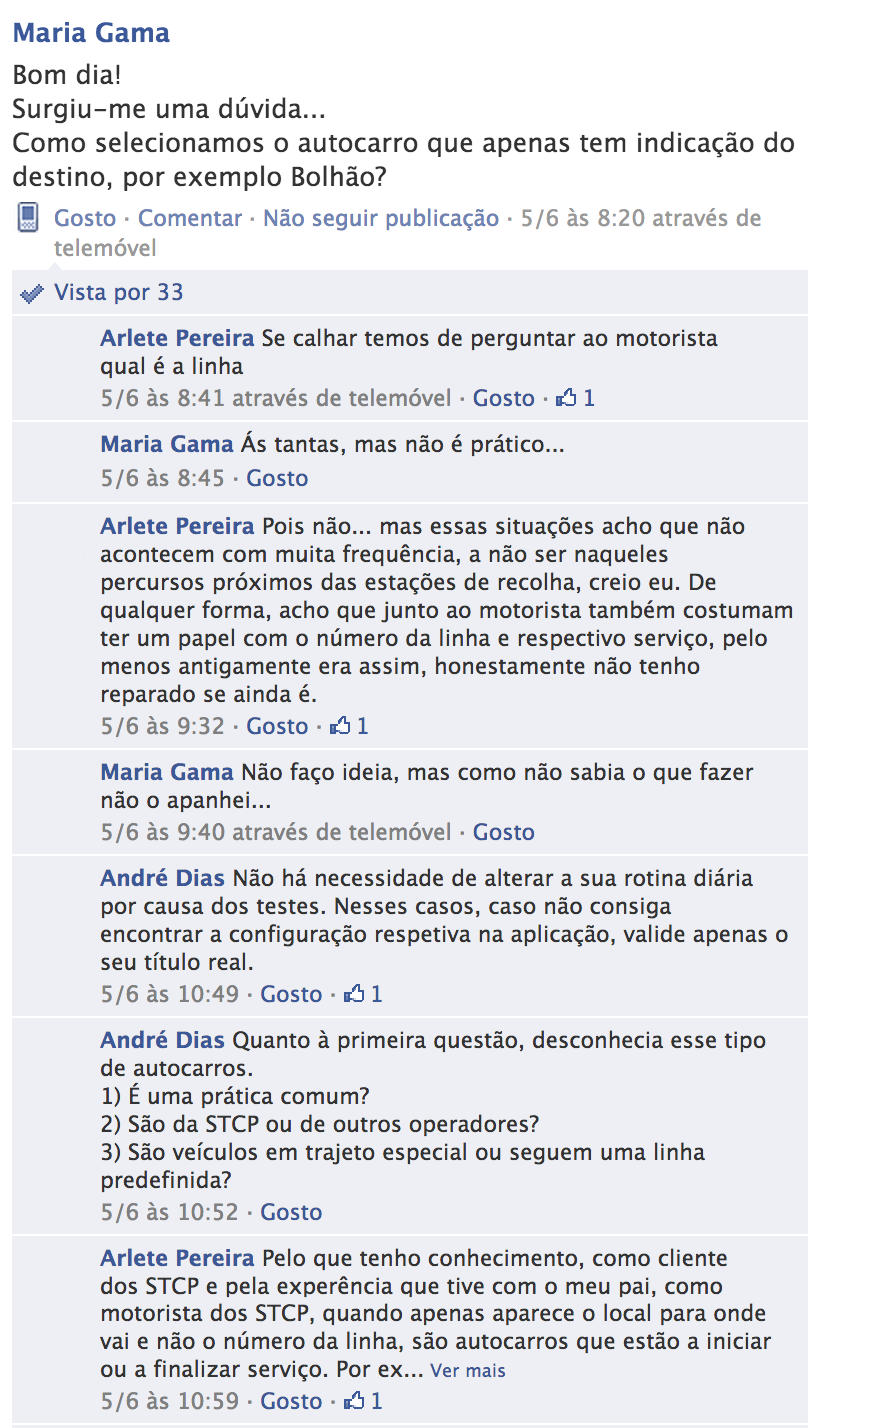
\includegraphics[height=23cm]{facebook1}
    \caption{Grupo Facebook}
    \label{facebook1}
  \end{center}
\end{figure}

\begin{figure}[t]
  \begin{center}
    \leavevmode
    
\includegraphics[height=15.9cm]{facebook2}
    \caption{Grupo Facebook}
    \label{facebook2}
  \end{center}
\end{figure}

\section{Testes MobiPag STCP}

Dos 37 utilizadores selecionados, 26 deram início ao teste da aplicação MobiPag STCP nos seus dispositivos, tendo a mesma sido disponibilizada via Google Play, em modo de teste (apenas utilizadores autorizados podem descarregar e instalar a aplicação). O processo de instalação decorreu sem problemas, havendo apenas alguma confusão devido ao facto de a aplicação não poder ser instalada diretamente da aplicação Play Store, sendo necessária uma aceitação prévia por parte do utilizador.
\\A aplicação foi disponibilizada dois dias antes do início dos testes, o que permitiu que os utilizadores efetuassem o registo e ambientação à aplicação de forma gradual e esclarecendo possíveis dúvidas. Devido a este facto, no dia em que os testes tiveram início, os utilizadores já estavam familiarizados com a aplicação e já sabiam como proceder nas várias ações a realizar.
\\Foi também marcada uma sessão presencial de esclarecimento de dúvidas, nas instalações da \Feup, um dia antes do início dos testes.

~\\O procedimento do teste era simples: replicar no dispositivo móvel as ações que efetuam no dia-a-dia com o cartão Andante. Comprar os mesmos títulos na aplicação que compram no sistema atual e, aquando da validação dos mesmos, efetuar também a sua validação no dispositivo móvel. Como se trata ainda de um protótipo, os títulos utilizados na aplicação são virtuais, não tendo qualquer valor legal, sendo por isso necessário validar obrigatoriamente os títulos reais, sob pena de incorrer em multa.

%%%%%%% atualizar número de validações %%%%%%%
~\\Durante o período de testes, os utilizadores realizaram cerca de 600 validações, em cerca de 215 paragens diferentes e cerca de 100 trajetos diferentes. Foram compradas 22 assinaturas mensais e realizadas cerca de 50 compras de um ou mais títulos de viagem ocasionais de várias tipologias. Apesar de a amostra ser pequena, foi possível obter algumas conclusões, nomeadamente a nível de alterações ao percurso habitual, que necessitam de ser previstas pela aplicação; paragens que não estão assinaladas na base de dados que suporta a aplicação; veículos que, por estarem a deslocar-se de/para a recolha, não possuem indicação do número da linha; paragens onde passam os dois sentidos da linha e portanto ser necessário especial cuidado na validação, sob pena de se validar no sentido contrário.

~\\Os utilizadores conseguiram realizar todas as operações sem dificuldade, embora o processo de validação tenha sido o mais apontado como necessário a melhorar. 
\\Em primeiro lugar, verificou-se que a localização através do GPS demora algum tempo e nem sempre as condições são as melhores. Já a localização através das redes móveis provou, em muitos casos, ser pouco precisa. Isto levou a que na maior parte dos casos fosse necessário recorrer à seleção manual das paragens (que estava pensada para ser utilizada apenas em casos pontuais), fazendo com que fosse necessário um passo extra no processo de validação.
\\O facto de não haver um histórico ou listagem de favoritos de paragens, obrigou a que de cada vez que quisessem efetuar uma validação, os utilizadores fossem obrigados a percorrer a lista de operadores, seguidamente a lista de linhas e depois então a paragem que pretendiam. Isto consome, obviamente, tempo num processo que se pretende o mais rápido possível.
\\Em algumas zonas onde a densidade de paragens é maior, nem sempre foi fácil para o utilizador identificar a paragem onde se encontrava. Em alguns casos de chegada à paragem ao mesmo tempo do que o veículo, não foi possível visualizar o código SMS da paragem e identificá-la de forma inequívoca.
\\Um outro fator apontado foi o de atualmente não ser necessária nenhuma operação, basta encostar o cartão no validador e o título está ativado. Posto isto, todo o processo de validação no dispositivo móvel deve ser o mais simples possível e com menor número de interações possível. Alguns utilizadores sugeriram repensar o método de validação, recorrendo, por exemplo, a QR Codes ou NFC nos veículos ou paragens.

~\\No que toca à fiscalização, não ocorreu nenhum problema, os fiscais estavam informados da ocorrência dos testes, fiscalizaram alguns dos utilizadores e obtiveram a informação necessária. Nesta fase de testes, a fiscalização é meramente visual, o que pode levar a alguns casos de fraude, sendo no futuro necessário acrescentar alguma segurança, por exemplo, dotando os fiscais com dispositivos de leitura e comunicação com o servidor.

~\\No decorrer dos testes, foi lançada uma versão atualizada da aplicação, com correção de alguns erros e implementação de uma nova funcionalidade. A lista de alterações é a seguinte:
\begin{itemize}
\item A seleção manual de paragens foi corrigida (nem sempre ficava selecionada a paragem correta);
\item No menu Histórico Validações foi corrigido um caracter na palavra “Validações”;
\item Informação das zonas da assinatura já não aparece truncada no saldo de títulos;
\item Implementado um histórico de paragens em que aparecem sempre as 2 últimas;
\item Corrigido o erro em que a aplicação encerrava se não tivesse nenhum fornecedor de localização ativo.
\end{itemize}

\section{Sugestões}
\label{sec:sugestoes}

Em termos de usabilidade, estes testes foram bastante úteis para perceber onde estavam as falhas e onde se pode melhorar. Os utilizadores foram bastante proativos e partilharam bastantes sugestões de funcionalidades ou melhorias que gostariam de ver implementadas. Algumas das sugestões apontadas são:
\begin{itemize}
\item Incluir os descontos sociais na compra da assinatura mensal;
\item Utilizar o Google Maps para melhor visualização das paragens;
\item Poder guardar um histórico de paragens;
\item Poder selecionar uma fotografia armazenada no telemóvel, removendo a necessidade de tirar a fotografia no momento do registo ou nas definições;
\item Verificar os campos sensíveis através de dupla verificação, de modo a evitar erros de introdução;
\item Traduzir a aplicação para outros idiomas (Inglês, Francês, etc.);
\item Listar as paragens por diferentes ordens (alfabética ou por sentido da linha);
\item Poder selecionar paragens favoritas;
\item Poder recuperar ou alterar a password;
\item Impor um limite de tentativas de autenticação via PIN;
\item Pesquisar paragens por código SMS ou nome;
\item Tornar o fundo do Menu Revisor mais legível;
\item Adicionar o destino na escolha das linhas;
\item Visualizar graficamente as zonas da assinatura no processo de compra;
\item Criar uma alternativa de fiscalização para quando o dispositivo fica sem bateria.
\item Facilitar o processo de validação através de QR Codes ou NFC;
\item Fornecer informação de horários, disponível na aplicação MOVE-ME;
\item Poder, de forma remota, fazer \emph{logout} da aplicação;
\item Criar vários parâmetros de personalização, nas definições da aplicação;
\item Possibilitar a renovação da assinatura mensal, não sendo necessário selecionar novamente as zonas incluídas na assinatura.
\end{itemize}